\chapter{From Minimum Wage to Real Estate Millionaire}

These notes follow Alex Kaufman's interview with School of Hard Knocks in the series \emph{10 Questions with a Millionaire}, curated by LazyingArt LLC through Video2Book. The subject is not blackboard physics, but it still has a serious quantitative structure. Income is redirected toward ownership; ownership creates equity; equity can create both liquidity and continuing cash flow; and risk is treated as a comparison between possible downside and forfeited upside. We keep the interview's order: the personal bottom, the business definition, the legal path into real estate, the first deal, the partnership, and finally the operating philosophy.

\section{The Reversal Before The Resume}

The interview begins with the hardest fact before the formal credentials. Alex says that from about age eleven to twenty-one he was under the influence of alcohol and drugs, and that by twenty-one he was a heroin addict. Only after that does the host reset the scene: this is episode five of \emph{10 Questions with a Millionaire}, and Alex is introduced as a real estate brokerage owner and real estate investor.

The order matters. The story is not introduced as a clean business ascent. It starts as a conversion problem:

\begin{equation}
\text{destructive path}
\quad \longrightarrow \quad
\text{sobriety}
\quad \longrightarrow \quad
\text{legal enterprise}.
\end{equation}

Once the interview settles into the business frame, Alex gives the first scale markers. He says he got started in real estate about five years earlier with his partner, Matt Teifke. They began by investing together, then partnered on the brokerage side, grew in Texas, and set the goal of building a global real estate brokerage for entrepreneurs. At the time of the interview, Alex says that he and Matt own approximately

\begin{equation}
U_{\text{owned}} \approx 100
\end{equation}

units together. The first measurable endpoint is not salary. It is ownership.

\section{The Brokerage As A Multi-Lane Skill Stack}

The host next asks what Alex means by ``entrepreneur.'' Alex answers by contrasting TRE's model with a conventional brokerage path. In the ordinary path, a new real estate licensee may be trained to do one thing: be a listing agent, be a buyer's agent, work residential, work commercial, or stay away from investing and wholesaling. Alex's objection is not that these individual skills are bad. His objection is that being confined to one lane makes a person fragile.

Let us call the possible real estate channels

\begin{equation}
\mathcal{C}
=
\{\text{listing},\text{buyer agency},\text{residential},\text{commercial},\text{investing},\text{wholesaling}\}.
\end{equation}

A narrow brokerage path gives the agent access to only a small subset of \(\mathcal{C}\). Alex's version of the real estate entrepreneur is someone trained to make money ``in and on'' real estate across more of the set.

\begin{figure}
\centering
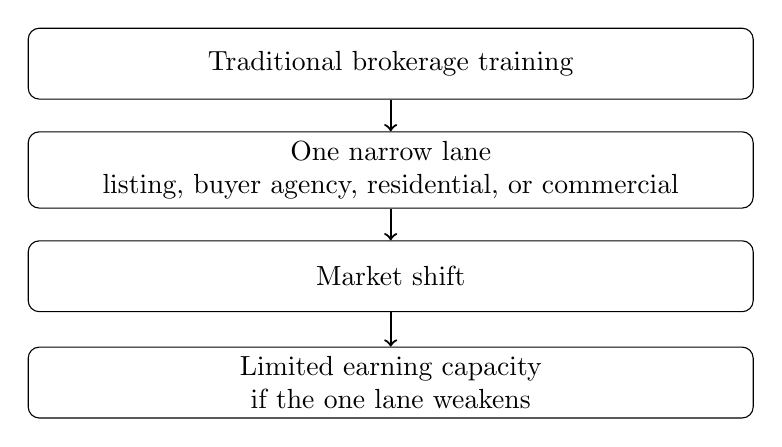
\begin{tikzpicture}[
  box/.style={draw, rounded corners, align=center, text width=0.74\linewidth, minimum height=0.9cm},
  arrow/.style={->, thick}
]
\node[box] at (0,0) (traditional) {Traditional brokerage training};
\node[box] at (0,-1.35) (lane) {One narrow lane\\listing, buyer agency, residential, or commercial};
\node[box] at (0,-2.70) (shift) {Market shift};
\node[box] at (0,-4.05) (limit) {Limited earning capacity\\if the one lane weakens};

\draw[arrow] (traditional) -- (lane);
\draw[arrow] (lane) -- (shift);
\draw[arrow] (shift) -- (limit);
\end{tikzpicture}
\caption{The narrow-path risk in Alex's account: specialization can become fragile when the market changes.}
\end{figure}

\subsection{Question \& Answer}

\paragraph{Question.}
Why is being taught only one real estate lane a business risk?

\paragraph{Answer.}
Because the market may stop rewarding that lane. If an agent has only one way to earn, then a market shift changes not only the market but the agent's usable skill set. In Alex's language, the better target is a ``true real estate professional'' who is not limited to one activity.

A cautious way to write the mechanism is

\begin{equation}
\text{earning capacity}
\approx
f(\text{usable channels},\ \text{market condition},\ \text{execution}).
\end{equation}

This is not a theorem. It is the business logic Alex is laying down: the broader the usable channel set, the more room a person has to adapt.

\section{Sobriety, Minimum Wage, And The Legal Money Path}

After defining the brokerage philosophy, the host asks for Alex's career path. The answer returns us to the opening reversal. Alex got sober at twenty-one. He worked at Firehouse Subs for

\begin{equation}
w_{\text{Firehouse}} = \$8.50/\text{hour}.
\end{equation}

He then washed dishes at a country club, worked in the kitchen, and worked for an oil and gas company. The point is not merely that these jobs were low-status or low-wage. The point is that they put pressure on a question that had become unavoidable after sobriety: if he believed he could make money for himself, how could he now do it legally?

That question moves the story to Matt Teifke. Alex says he had known Matt since he was about eight years old, and Matt showed him the path in real estate. The first bridge into the asset world is therefore not a textbook or a credential. It is a relationship with someone who already had domain judgment.

\section{Matt, Trust, And The First Deal}

When the host asks how Alex moved from starting in real estate to owning a brokerage, Alex clarifies that Matt is the licensed broker, but the two of them own the brokerage together. TRE is presented as a deliberate counter-model to the narrow brokerage path discussed earlier. They wanted a place where people could get more out of real estate for themselves.

At that stage, Alex says they had already been buying real estate together and owned about fifteen units. The sequence is useful:

\begin{enumerate}
\item They begin by investing together.
\item They see the limits of conventional brokerage training.
\item Matt has the broker license.
\item They form TRE as a brokerage for real estate entrepreneurs.
\end{enumerate}

The transcript becomes garbled just before the first-deal story, so we use only the clear claims. Alex says he had never bought real estate before. A figure of about \(\$28{,}000\) appears. Matt tells him to trust the deal. Alex says he put his trust in Matt's judgment. Later, Alex describes the property as worth close to \(\$400{,}000\), says they pulled about \(\$150{,}000\) out of it, and says they still own it and collect rent every month.

\subsection{Question \& Answer}

\paragraph{Question.}
How could the first deal happen when Alex had never bought real estate before?

\paragraph{Answer.}
In this particular story, missing experience was partly bridged by trusted partnership. Matt supplied the domain judgment; Alex supplied action and trust. That is not a universal replacement for underwriting. It is the local mechanism by which the first acquisition became possible:

\begin{equation}
\text{first action}
=
\text{trust}
+
\text{available capital}
+
\text{partner's judgment}.
\end{equation}

The point is not that trust removes risk. The point is that, for Alex, trust made action possible before he had his own long record of real estate decisions.

\section{The First Deal As A Wealth Mechanism}

Now the strongest quantitative part of the interview comes into view. Let \(C_0\) denote the stated first-deal cash figure. We do not know whether this was a down payment, total cash needed, a contribution, or another capital figure, so the notation should stay neutral:

\begin{equation}
C_0 \approx \$28{,}000.
\end{equation}

Let \(V_{\text{later}}\) denote Alex's spoken estimate of the later property value:

\begin{equation}
V_{\text{later}} \approx \$400{,}000.
\end{equation}

Let \(E_{\text{out}}\) denote the amount he says they pulled out while still owning the property:

\begin{equation}
E_{\text{out}} \approx \$150{,}000.
\end{equation}

A rough scale comparison is useful if we keep it honest:

\begin{align}
\frac{V_{\text{later}}}{C_0}
&\approx
\frac{400{,}000}{28{,}000} \\
&\approx 14.3.
\end{align}

This is not a net return, an annualized return, or an equity multiple. The transcript does not give the purchase price, debt, repairs, taxes, interest, closing costs, operating expenses, or precise timing. The ratio only tells us that the later stated property value was about \(14.3\) times the stated initial cash figure.

\subsection{A Worked Mechanism}

The important feature is not only appreciation. It is retained ownership. The mechanism, as stated in the interview, runs as follows:

\begin{enumerate}
\item Capital is committed:
\[
C_0 \approx \$28{,}000.
\]

\item A property is acquired and held.

\item Alex later estimates the property's value near
\[
V_{\text{later}} \approx \$400{,}000.
\]

\item Value is extracted:
\[
E_{\text{out}} \approx \$150{,}000.
\]

\item The property remains owned and continues producing monthly rent cash flow.
\end{enumerate}

So the wealth effect is not simply ``buy low, sell high.'' In Alex's telling, it is closer to

\begin{equation}
\text{wealth effect}
\approx
\text{retained ownership}
+
\text{extracted equity}
+
\text{monthly cash flow}.
\end{equation}

That is the real estate mechanism the interview preserves: a first cash commitment becomes an asset; the asset can later support liquidity; and ownership can remain in place.

\begin{figure}
\centering
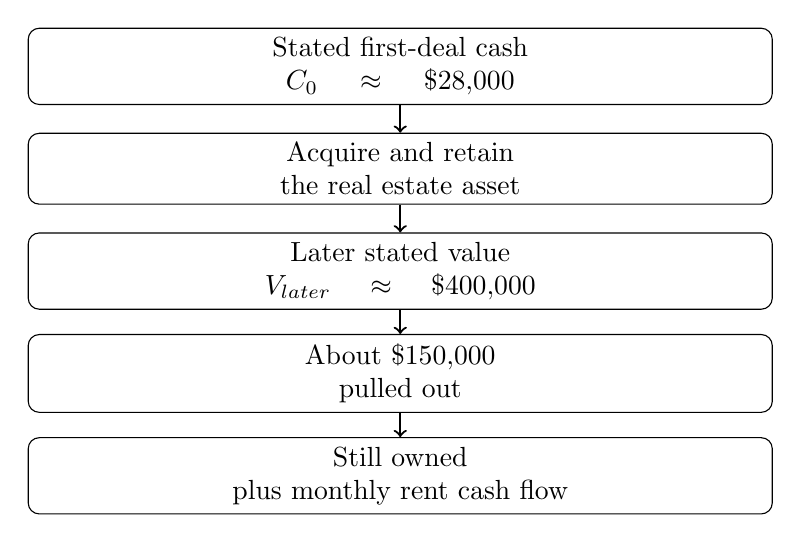
\begin{tikzpicture}[
  box/.style={draw, rounded corners, align=center, text width=0.76\linewidth, minimum height=0.9cm},
  arrow/.style={->, thick}
]
\node[box] at (0,0) (cash) {Stated first-deal cash\\\(C_0 \approx \$28{,}000\)};
\node[box] at (0,-1.30) (acq) {Acquire and retain\\the real estate asset};
\node[box] at (0,-2.60) (value) {Later stated value\\\(V_{\text{later}} \approx \$400{,}000\)};
\node[box] at (0,-3.90) (extract) {About \(\$150{,}000\)\\pulled out};
\node[box] at (0,-5.20) (keep) {Still owned\\plus monthly rent cash flow};

\draw[arrow] (cash) -- (acq);
\draw[arrow] (acq) -- (value);
\draw[arrow] (value) -- (extract);
\draw[arrow] (extract) -- (keep);
\end{tikzpicture}
\caption{A transcript-derived reconstruction of the first-deal mechanism. The interview does not specify the financing structure.}
\end{figure}

\section{Partnership: Same Values, Different Work}

The host then moves from the first asset to the partnership itself. Alex does not describe the partnership as something designed all at once. They did deals together. They worked together. He learned from Matt, did legwork, took action, and helped find deals while Matt had his own commercial brokerage and property-management context.

The rule that emerges has two parts. First, partners need shared values, trust, goals, and vision. Alex is explicit that moral and value misalignment will create conflict later. Second, partners should not merely duplicate each other. Matt is described as strong in sales, networking, relationships, ideas, and vision. Alex describes himself as drawn to execution: putting plans into action, running the business, running operations, and growing and scaling operations.

\begin{table}
\centering
\begin{tabular}{|p{0.42\linewidth}|p{0.42\linewidth}|}
\hline
Matt Teifke & Alex Kaufman \\
\hline
Sales & Operations \\
Networking & Execution \\
Meeting people & Running the business \\
Relationships & Operational growth \\
Ideas and vision & Scaling systems \\
\hline
\end{tabular}
\caption{The complementary partnership roles described in the interview.}
\end{table}

We can summarize the operating condition as

\begin{equation}
\text{strong partnership}
\approx
\text{shared values}
+
\text{trust}
+
\text{complementary skills}.
\end{equation}

Alex adds an important qualification. Being close like family does not automatically make people good business partners. In his account, the strength came from having both: brother-like trust and useful business complementarity.

\section{Risk, Reinvestment, And The Cost Of Inaction}

The next question compresses the experience into financial judgment: what was the best financial decision, and what was the worst? Alex says the best was putting every penny he made into real estate and into the businesses. The worst, he says, was not taking more risks.

That answer creates the section's local puzzle.

\subsection{Question \& Answer}

\paragraph{Question.}
How can avoiding risk still be risky?

\paragraph{Answer.}
Avoiding an investment can reduce one exposure: the possibility of losing the money committed to that investment. But it creates another exposure: the missed upside from never acting. Alex states this as a practical rule. By not putting money into an investment, one may be risking the rewards that would have come from the upside.

A compact way to separate the two sides is

\begin{equation}
\text{risk of action}
=
\text{possible downside},
\end{equation}

while

\begin{equation}
\text{risk of inaction}
=
\text{forfeited upside}.
\end{equation}

Neither side is automatically dominant. The point is that inaction has a payoff structure too. Safety is not the same as neutrality.

Alex's own operating claim is more aggressive than a general portfolio rule. He says they put everything on the line and carry complete belief that they will make it work. We should read that as his style of entrepreneurship, not as universal financial advice. The general mechanism is opportunity cost; the personal claim is high-conviction reinvestment.

\begin{equation}
\text{income}
\quad \longrightarrow \quad
\text{real estate and business}
\quad \longrightarrow \quad
\text{expanded ownership capacity}.
\end{equation}

This connects back to the first deal. Money is not treated as the endpoint. It is treated as fuel for more assets, more operating capacity, and more deal flow.

\section{Vision, Sacrifice, And What The Number Is For}

When asked where he sees himself in ten years, Alex does not give a unit count, a cash-flow number, a revenue target, or a profit target. He says that is not the kind of number he and Matt have fixed. The goal is a community and network of entrepreneurs under Teifke Real Estate across the world, doing deals, helping each other, and growing together. The Mars joke at the end of this answer keeps the ambition informal, but the mechanism is clear: the future target is a network, not merely a balance-sheet number.

Earlier, the numbers mattered because they showed the first asset mechanism. Here, the absence of a number matters. The stated target is not

\begin{equation}
\text{goal}
=
\text{fixed unit count}
\quad \text{or} \quad
\text{fixed revenue}.
\end{equation}

It is closer to

\begin{equation}
\text{goal}
=
\text{network}
+
\text{community}
+
\text{deal flow}
+
\text{mutual help}.
\end{equation}

The final advice returns to personal responsibility. Alex says personal situations differ. When he was working at Firehouse Subs and other jobs, he had no wife, no children, and no one relying on him; that gave him room to take actions that someone with heavier obligations might not be able to take. Still, his broader claim remains demanding: if one wants something badly enough, one has to figure out a way, sacrifice for it, stop letting outside voices define the boundary of possibility, and become fully accountable to oneself.

So the lecture ends where it began, with redirection. The desire to make money is not enough. It has to be placed inside legality, sacrifice, ownership, trust, operating skill, and responsibility.

\section{Summary}

Alex Kaufman's interview is built around a sequence of conversions. Personal disorder is converted into sobriety. Minimum-wage work is converted into the search for legal self-directed earning. A childhood relationship with Matt Teifke becomes a bridge into real estate. A stated \(\$28{,}000\) first-deal cash figure becomes, in Alex's account, a property later worth close to \(\$400{,}000\), with about \(\$150{,}000\) pulled out while ownership and monthly rent continue.

The durable lesson for the larger book is structural, not imitative. The transcript does not provide enough financing detail to copy the exact deal. What it does provide is a mechanism: move from labor income toward ownership, from one-lane work toward multiple earning channels, from isolated ambition toward trusted partnership, and from passive safety toward calculated exposure to upside.